\documentclass[a4paper,11pt,pdf]{../templates/pacmanreport}

%%=== Aditional packages


%%=== Local definitions
\graphicspath{{images/}{../shared_images/}}

%% ================================
%% PROJECT INFO 

\project{}
\projectid{FP7-IST-60918}
\projectstart{1 March 2013}
\duration{36}

%% ================================
%% DELIVERABLE INFO 

\title{Planning Active Information Gathering for Haptic and Vision}
\deliverableid{DR 3.2}
\author{C. Zito, C. Rosales, F. Spinelli, A. Rietzler, J. L. Wyatt}
\address{School of Computer Science, University of Birmingham}
\email{claudio.zito.81@gmail.com}
\headertitle{Active Information Gathering}
\headerauthor{C. Zito, C. Rosales, F. Spinelli, A. Rietzler, J. L. Wyatt}

\duedate{2015-02-27}
\submissiondate{2015-02-27}
\leadpartner{BHAM}
\revision{draft}
\disseminationlevel{PU}


%% UNCOMMENT: to get the logo; if you've copied this file to a directory yearX/wpY/ then this should work
\reportlogo{pacmanlogo}


\begin{document}

\maketitle

\begin{abstract}
\noindent 
This report describes activities related to the development of planning algorithms for actively gathering information for object of unknown shape. This report presents the efforts on the definition of information theoretic measures for uncertainty about shape as well as modelling of incomplete surfaces. It also describes how to integrate low-level controllers, developed on Task 3.1, to plan haptic exploration strategies for a bi-manual robot which holds in one hand an unknown object and is capable of tracing the object's surface with a sensorised finger.  


\end{abstract}


\vspace{.2em}
\hrule

\footnotesize

\tableofcontents

\normalsize

\newpage

\section*{Executive Summary}

This report describes the activities within the PaCMan consortium to define methodologies for \emph{active information gathering}.
The material included in this report presents results on reactive control strategies for haptic exploration developed in Task 3.1 (M 1-18) as well as results on planning and execution of active visual information gathering developed in Task 3.3 (M 1-36).

\section*{Role of active information gathering in PaCMan}

This deliverable presents the achievements of the consortium in the development of new strategies for planning of active information gathering actions. 

\section*{Contribution to the PaCMan scenario}

Robot grasping is typically affected by uncertainty associated to the location of the object to be grasped as well as its shape. A robot could gather information either by i) touching the object or ii) visually observing it from different point of views. This report presents three approaches that enable a robot to reason about such uncertainties and to plan the best-next action to maximise the information gain.


\newpage

\section{Tasks, objectives, results}

\subsection{Planned work}

This deliverable addresses the work developed in Task 3.2 and Task 3.3. In particular, the development of planning active strategies for information gathering through both vision and haptic exploration of unknown objects. This includes using vision and haptic clues to build probabilistic models of the object to be manipulated.   

\subsection{Actual work performed}

\subsection{Task 3.2}

This task addresses the problem of planning and execute active information gathering for objects of unknown shape. Our solution employs a Gaussian Process (GP) for estimating an implicitly-defined function as well as provide a measurement of the uncertainty on the estimated surface. The approximating function can be considered as the 0-levelset of the surface of the object to be manipulated, it comes handy to interpret it as a manifold and to build on recent developments on sample-based techniques for manifold explorations, e.g.~\cite{Jaillet2013Path}. We extend such algorithms to define the next-best exploration action to minimise the reduction of shape uncertainty. 

The work in~\cite{Dragiev2011Gaussian} is one of the first attempt to employ GP for implicit surfaces for representing shapes in tasks as robotic grasping. However, the authors rely only on the MAP estimation of the surface (its mean) without exploiting the model uncertainty. The same authors in~\cite{Dragiev2013Uncertainty} extended their previous work to formulate a way to make inference from the GP to prefer regions on the model with particular certainty level and introduce the concept of explore-grasp and exploit grasp primitives. 

Our proposed solution has several advantages: i) it implicitly defines the unknown shape in a probabilistic model, ii) integrates visual and haptic information in its model to refine its predictions and iii) constructs paths on the object's surface that a robot equipped with a sensorised finger can follow in order to gather haptic information. 
The algorithm is demonstrated in simulation and on a real robotic platform (Vito) where a bi-manual robot holds an unknown object in its hand and it is cabable of tracing the object surface with the other arm equipped with a F/T sensor.
%do we have a paper to cite about the probe finger?

The experimental results show that our framework can learn the object shape and yields to better models with a reduced number of exploration actions.

\subsection{Relation to the state-of-the-art}



How are the obtained results related to the state-of-the-art? 

\bibliographystyle{ieeetr}
\bibliography{../shared_bibliography/abbreviations,./bibliography/DR32}

\newpage

\appendix
\section{Annexes}

Which papers / articles are included in the report? Mention titles, authors, publication info; abstract; and a one-liner relating the publication back to the discussion on actual work performed. 

% template for annexes
\subsection{Book chapter/Article/Technical Report: \em TITLE}
\begin{description}
    \item[Authors] 
    \item[Info] % UNDER REVIEW / IN PRESS / ACCEPTED FOR PUBLICATION (PROVIDE WHERE) / PUBLISHED AND AVAILABLE ONLINE (PROVIDE DOI)
    \item[Abstract]
    \item [Relation with the deliverable] 
    \item[Attachment] %if so, e.g. (following pages until next annex) or The article can be downloaded at the DOI link above, hence no attachment is provided
\end{description}
% attach your PDF(s) if required, pusblished and online available documents do not require it if you provide the doi (only doi are permitted)
%\includepdf[pages=-]{./attachedPapers/YOURFILE.pdf

\subsection{Technical Report: \em The Next Best Touch or Non-Touch:
Object Pose Estimation via Sculpting with Compliant Hands}
\begin{description}
    \item[Authors] Alexander Rietzler, Carlos J. Rosales, Marco Gabiccini, Justus Piater
    \item[Info] Paper Draft% UNDER REVIEW / IN PRESS / ACCEPTED FOR PUBLICATION (PROVIDE WHERE) / PUBLISHED AND AVAILABLE ONLINE (PROVIDE DOI)
    \item[Abstract] Many robotic tasks rely on the ability of a vision system to accurately estimate the 6 dimensional pose of objects in a scene.
In many cases a single vision sensor does not provide sufficient information to discriminate a single correct
pose of an object. 
This paper solves the problem of refining the pose distribution 
of an object solely via proprioceptive sensing of occupancy.
Our main novel contribution is an algorithm that plans a robot arm-hand trajectory such that 
information gathered about the object pose belief is maximized while at the same time impact on the object is minimized. 
This may result in actions that do not make contact with the object at all.
Impact on the object is further reduced by using a compliant robotic hand.
    \item [Relation with the deliverable] This report reports work done under\\ Task~2.3 by introducing a method for reducing an object's pose uncertainty by performing proprioceptive information
    gathering actions.
    \item[Attachment] (following pages) %if so, e.g. (following pages until next annex) or The article can be downloaded at the DOI link above, hence no attachment is provided
\end{description}
% attach your PDF(s) if required, pusblished and online available documents do not require it if you provide the doi (only doi are permitted)
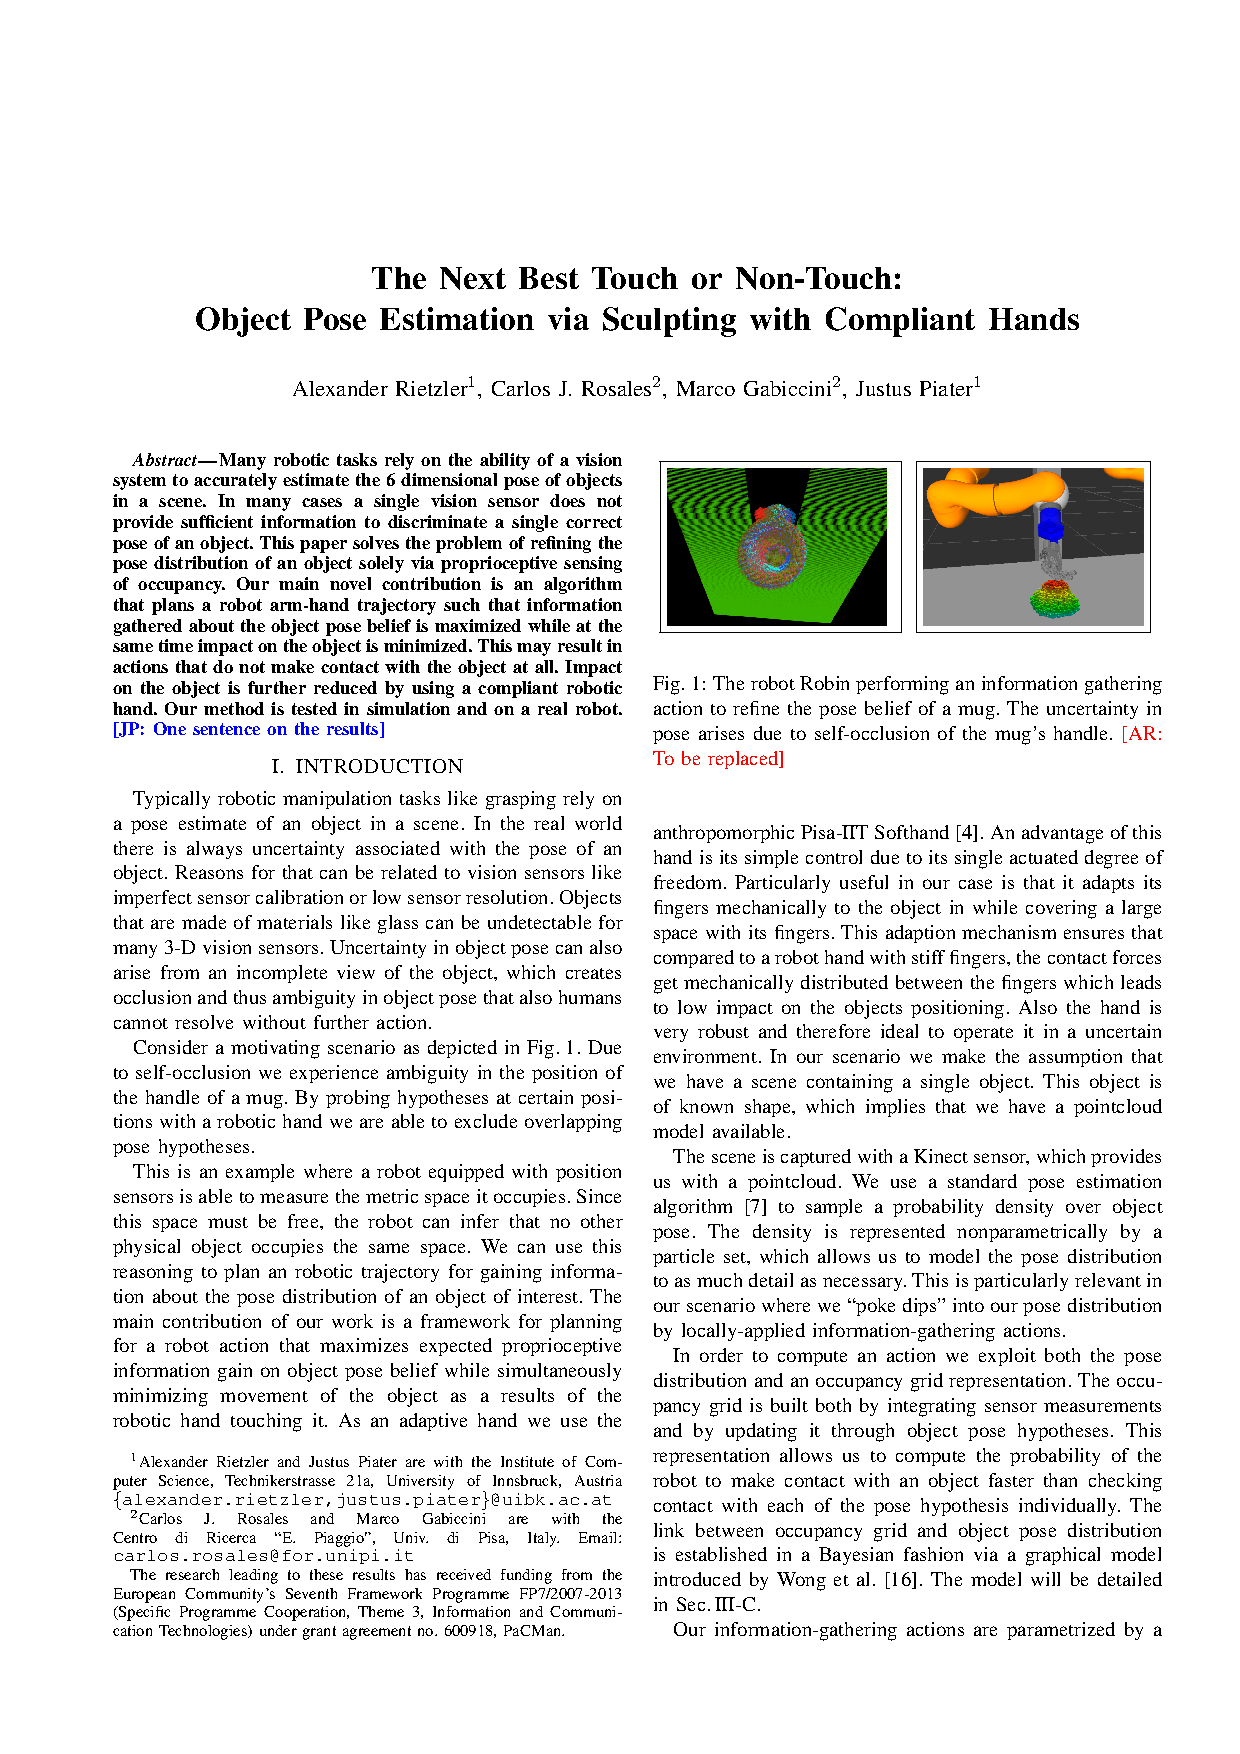
\includepdf[pages=-]{./attachedPapers/iros_draft_rietzleretal.pdf}


\end{document}
